% Généré par build/plot_ladders_main.py — ne pas éditer à la main.
% Source : results/control_usa_ladders_n20000.json (seed 20260827, 20000 traj.).
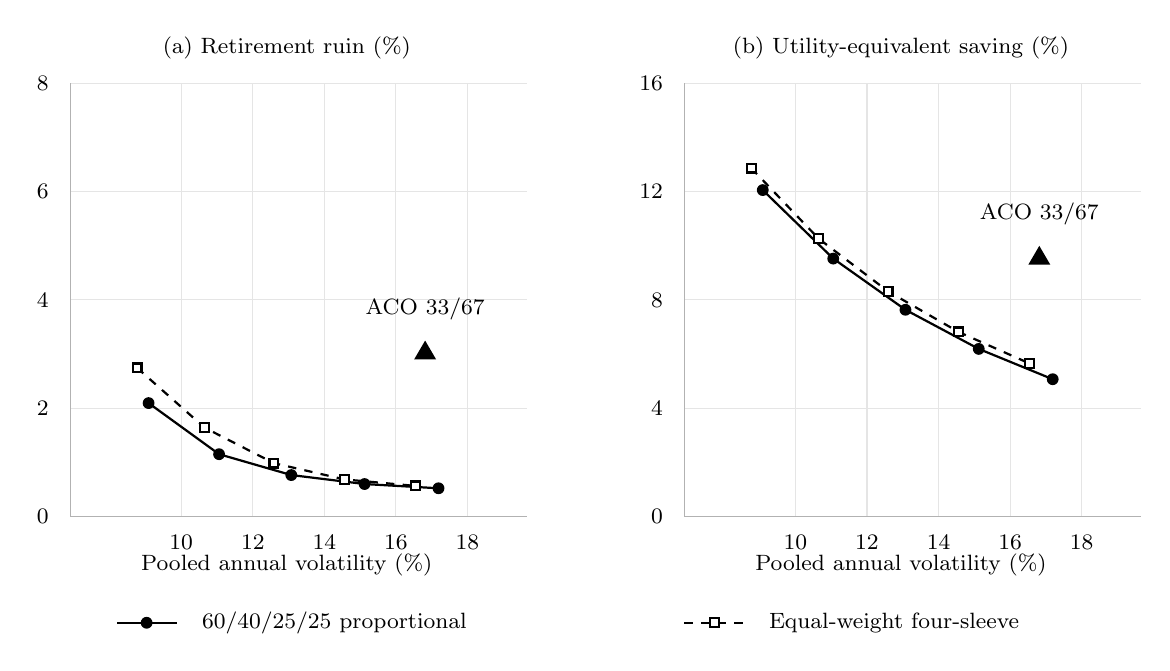
\begin{tikzpicture}[x=1cm, y=1cm]
\begin{scope}[shift={(0.0,0)}]
  \draw[gray!20] (0,0.000) -- (5.80,0.000);
  \node[left, font=\footnotesize] at (-0.15,0.000) {0};
  \draw[gray!20] (0,1.375) -- (5.80,1.375);
  \node[left, font=\footnotesize] at (-0.15,1.375) {2};
  \draw[gray!20] (0,2.750) -- (5.80,2.750);
  \node[left, font=\footnotesize] at (-0.15,2.750) {4};
  \draw[gray!20] (0,4.125) -- (5.80,4.125);
  \node[left, font=\footnotesize] at (-0.15,4.125) {6};
  \draw[gray!20] (0,5.500) -- (5.80,5.500);
  \node[left, font=\footnotesize] at (-0.15,5.500) {8};
  \draw[gray!20] (1.409,0) -- (1.409,5.500);
  \node[below, font=\footnotesize] at (1.409,-0.12) {10};
  \draw[gray!20] (2.318,0) -- (2.318,5.500);
  \node[below, font=\footnotesize] at (2.318,-0.12) {12};
  \draw[gray!20] (3.227,0) -- (3.227,5.500);
  \node[below, font=\footnotesize] at (3.227,-0.12) {14};
  \draw[gray!20] (4.136,0) -- (4.136,5.500);
  \node[below, font=\footnotesize] at (4.136,-0.12) {16};
  \draw[gray!20] (5.045,0) -- (5.045,5.500);
  \node[below, font=\footnotesize] at (5.045,-0.12) {18};
  \draw[gray!60] (0,0) -- (5.80,0);
  \draw[gray!60] (0,0) -- (0,5.500);
  \fill (4.507,2.234) -- ++(-0.14,-0.24) -- ++(0.28,0) -- cycle;
  \node[font=\footnotesize, anchor=south] at (4.507,2.374) {ACO 33/67};
  \draw[thick] plot coordinates {(0.995,1.440) (1.890,0.791) (2.807,0.526) (3.738,0.412) (4.677,0.358)};
  \fill (0.995,1.440) circle (0.075);
  \fill (1.890,0.791) circle (0.075);
  \fill (2.807,0.526) circle (0.075);
  \fill (3.738,0.412) circle (0.075);
  \fill (4.677,0.358) circle (0.075);
  \draw[thick, dashed] plot coordinates {(0.849,1.887) (1.706,1.128) (2.586,0.677) (3.480,0.471) (4.383,0.388)};
  \node[draw, thick, rectangle, inner sep=1.6pt, fill=white] at (0.849,1.887) {};
  \node[draw, thick, rectangle, inner sep=1.6pt, fill=white] at (1.706,1.128) {};
  \node[draw, thick, rectangle, inner sep=1.6pt, fill=white] at (2.586,0.677) {};
  \node[draw, thick, rectangle, inner sep=1.6pt, fill=white] at (3.480,0.471) {};
  \node[draw, thick, rectangle, inner sep=1.6pt, fill=white] at (4.383,0.388) {};
  \node[font=\footnotesize] at (2.75,5.95) {(a) Retirement ruin (\%)};
  \node[font=\footnotesize] at (2.75,-0.62) {Pooled annual volatility (\%)};
\end{scope}
\begin{scope}[shift={(7.8,0)}]
  \draw[gray!20] (0,0.000) -- (5.80,0.000);
  \node[left, font=\footnotesize] at (-0.15,0.000) {0};
  \draw[gray!20] (0,1.375) -- (5.80,1.375);
  \node[left, font=\footnotesize] at (-0.15,1.375) {4};
  \draw[gray!20] (0,2.750) -- (5.80,2.750);
  \node[left, font=\footnotesize] at (-0.15,2.750) {8};
  \draw[gray!20] (0,4.125) -- (5.80,4.125);
  \node[left, font=\footnotesize] at (-0.15,4.125) {12};
  \draw[gray!20] (0,5.500) -- (5.80,5.500);
  \node[left, font=\footnotesize] at (-0.15,5.500) {16};
  \draw[gray!20] (1.409,0) -- (1.409,5.500);
  \node[below, font=\footnotesize] at (1.409,-0.12) {10};
  \draw[gray!20] (2.318,0) -- (2.318,5.500);
  \node[below, font=\footnotesize] at (2.318,-0.12) {12};
  \draw[gray!20] (3.227,0) -- (3.227,5.500);
  \node[below, font=\footnotesize] at (3.227,-0.12) {14};
  \draw[gray!20] (4.136,0) -- (4.136,5.500);
  \node[below, font=\footnotesize] at (4.136,-0.12) {16};
  \draw[gray!20] (5.045,0) -- (5.045,5.500);
  \node[below, font=\footnotesize] at (5.045,-0.12) {18};
  \draw[gray!60] (0,0) -- (5.80,0);
  \draw[gray!60] (0,0) -- (0,5.500);
  \fill (4.507,3.437) -- ++(-0.14,-0.24) -- ++(0.28,0) -- cycle;
  \node[font=\footnotesize, anchor=south] at (4.507,3.577) {ACO 33/67};
  \draw[thick] plot coordinates {(0.995,4.145) (1.890,3.275) (2.807,2.625) (3.738,2.128) (4.677,1.743)};
  \fill (0.995,4.145) circle (0.075);
  \fill (1.890,3.275) circle (0.075);
  \fill (2.807,2.625) circle (0.075);
  \fill (3.738,2.128) circle (0.075);
  \fill (4.677,1.743) circle (0.075);
  \draw[thick, dashed] plot coordinates {(0.849,4.424) (1.706,3.527) (2.586,2.859) (3.480,2.344) (4.383,1.943)};
  \node[draw, thick, rectangle, inner sep=1.6pt, fill=white] at (0.849,4.424) {};
  \node[draw, thick, rectangle, inner sep=1.6pt, fill=white] at (1.706,3.527) {};
  \node[draw, thick, rectangle, inner sep=1.6pt, fill=white] at (2.586,2.859) {};
  \node[draw, thick, rectangle, inner sep=1.6pt, fill=white] at (3.480,2.344) {};
  \node[draw, thick, rectangle, inner sep=1.6pt, fill=white] at (4.383,1.943) {};
  \node[font=\footnotesize] at (2.75,5.95) {(b) Utility-equivalent saving (\%)};
  \node[font=\footnotesize] at (2.75,-0.62) {Pooled annual volatility (\%)};
\end{scope}
  \draw[thick] (0.60,-1.35) -- (1.35,-1.35);
  \fill (0.97,-1.35) circle (0.075);
  \node[font=\footnotesize, anchor=west] at (1.55,-1.35) {60/40/25/25 proportional};
  \draw[thick, dashed] (7.80,-1.35) -- (8.55,-1.35);
  \node[draw, thick, rectangle, inner sep=1.6pt, fill=white] at (8.18,-1.35) {};
  \node[font=\footnotesize, anchor=west] at (8.75,-1.35) {Equal-weight four-sleeve};
\end{tikzpicture}
